\documentclass{beamer}
\usetheme[compress]{Singapore}
\useoutertheme{miniframes}

% Packages nécessaires
%
% Pour les documents en fran�ais...
	\usepackage[utf8]{inputenc}
	\usepackage[french]{babel}    
	\usepackage[french]{varioref} 
	
% Math�matiques
	\usepackage{amsmath}
	
% Caracteres speciaux
        \usepackage{latexsym,amsfonts}	

% A documenter	
	\usepackage{moreverb}
	\usepackage{lipsum}

% Pour ins�rer des graphiques	
%	\usepackage{graphicx}	% Graphique simples
	\usepackage{eso-pic,graphicx}	% Graphique simples    
	\usepackage{subfigure}				% Graphiques multiples
	\usepackage{xcolor}
	\usepackage{tikz}
%	\usepackage{animate}

% Pour le sch�ma de latex...
	%\usepackage[active,tightpage]{preview} 	
	%\PreviewEnvironment{tikzpicture}			
	%\setlength\PreviewBorder{5pt}					
	\usetikzlibrary{positioning}						
	
% Pour ins�rer des couleurs	
	\usepackage{color}

% Outil suppl�mentaire pour les tableaux
	\usepackage{multirow}
 	\usepackage{booktabs}
	\usepackage{longtable}
	\usepackage{colortbl}
	
% Rotation des objets et des pages
	\usepackage{rotating}
	\usepackage{lscape}

% Pour ins�rer du code source, LaTeX ou SAS par exemple.
	\usepackage{verbatim}
	\usepackage{fancyvrb}
	\usepackage{listings} 
	\lstset{language=SAS,numbers=left}		% Par d�faut le listing est en SAS 

% Pour ins�rer des hyperliens
	\usepackage{hyperref}

% American Psychological Association (for bibliographic references).
	\usepackage{apacite}
  
% Pour l'utilisation des macros
	\usepackage{xspace}

% Pour l'utilisation de notes en fin de document.
	\usepackage{endnotes}

% Rotation
	\usepackage{rotating}

% Pour les t�ches de caf�
%	\usepackage{coffee}

% Symboles suppl�mentaires
	\usepackage{bbding}
	\usepackage{pifont}

% Pour les listes num�rot�es
%\usepackage{paralist}
	\usepackage{enumerate}
%\usepackage{enumitem}

% En t�tes et pieds de pages
 	\usepackage{fancyhdr}

% Pour le multi-colonne sous Beamer ?
	\usepackage{multicol}

% Pour la derni�re page
	\usepackage{lastpage}

% Pour Highlight d'Andre Simon
\usepackage{alltt}
%\usepackage[T1]{fontenc}

% Logos
\usepackage{mflogo}

%TikZ
  \usepackage{tikz}
  \usetikzlibrary{shadows,arrows}
  \pgfdeclarelayer{background}
  \pgfdeclarelayer{foreground}
  \pgfsetlayers{background,main,foreground}

% pour les symboles
\usepackage{keystroke}
%\usepackage{feyn}
\usepackage{bbding}
\usepackage{phonetic}
%% Macros commandes
%
% Pour ins�rer des dessins de Linux
\newcommand{\LinuxA}{\includegraphics[height=0.5cm]{Graphiques/linux.png}}
\newcommand{\LinuxB}{\includegraphics[height=0.5cm]{Graphiques/linux.png}\xspace}

% Macro pour les petits dessins pour les diff�rents OS.
\newcommand{\Windows}{\emph{Windows}\xspace}
\newcommand{\Mac}{\emph{Mac OS X}\xspace}
\newcommand{\Linux}{\emph{Linux}\xspace}
\newcommand{\MikTeX}{MiK\tex\xspace}

% Des raccourcis pour les commandes \LaTeX, \TeX, ...
\newcommand{\latex}{\LaTeX\xspace}
\newcommand{\latexe}{\LaTeXe\xspace}
\newcommand{\tex}{\TeX\xspace}

% Commande pour le mode Verbatim
%\newcommand{\code}{\vspace{0.2cm}\begin{Verbatim}[frame=single,label=Code,fontsize=\small]}
%\newcommand{\tinycode}{\vspace{0.2cm}\begin{Verbatim}[frame=single,label=Code,fontsize=\tiny]}
%
%% From Framabook (www.framasoft.net)
%\newcommand{\latexcom}[1]{{\mdseries\ttfamily\upshape\symbol{92}#1}}
%\newcommand{\indexcom}[1]{%
  %\index{#1@\protect\texttt{\symbol{92}#1}}}
%\newcommand{\ltxcom}[1]{%
  %\latexcom{#1}\indexcom{#1}}  
%
  %\newcommand{\yslant}{0.5}
%\newcommand{\xslant}{-0.6}

% knitr
\usepackage[]{graphicx}\usepackage[]{color}
%% maxwidth is the original width if it is less than linewidth
%% otherwise use linewidth (to make sure the graphics do not exceed the margin)
%\makeatletter
%\def\maxwidth{ %
  %\ifdim\Gin@nat@width>\linewidth
    %\linewidth
  %\else
    %\Gin@nat@width
  %\fi
%}
%\makeatother

\definecolor{fgcolor}{rgb}{0.345, 0.345, 0.345}
\newcommand{\hlnum}[1]{\textcolor[rgb]{0.686,0.059,0.569}{#1}}%
\newcommand{\hlstr}[1]{\textcolor[rgb]{0.192,0.494,0.8}{#1}}%
\newcommand{\hlcom}[1]{\textcolor[rgb]{0.678,0.584,0.686}{\textit{#1}}}%
\newcommand{\hlopt}[1]{\textcolor[rgb]{0,0,0}{#1}}%
\newcommand{\hlstd}[1]{\textcolor[rgb]{0.345,0.345,0.345}{#1}}%
\newcommand{\hlkwa}[1]{\textcolor[rgb]{0.161,0.373,0.58}{\textbf{#1}}}%
\newcommand{\hlkwb}[1]{\textcolor[rgb]{0.69,0.353,0.396}{#1}}%
\newcommand{\hlkwc}[1]{\textcolor[rgb]{0.333,0.667,0.333}{#1}}%
\newcommand{\hlkwd}[1]{\textcolor[rgb]{0.737,0.353,0.396}{\textbf{#1}}}%

%\usepackage{framed}
%\makeatletter
%\newenvironment{kframe}{%
 %\def\at@end@of@kframe{}%
 %\ifinner\ifhmode%
  %\def\at@end@of@kframe{\end{minipage}}%
  %\begin{minipage}{\columnwidth}%
 %\fi\fi%
 %\def\FrameCommand##1{\hskip\@totalleftmargin \hskip-\fboxsep
 %\colorbox{shadecolor}{##1}\hskip-\fboxsep
     %% There is no \\@totalrightmargin, so:
     %\hskip-\linewidth \hskip-\@totalleftmargin \hskip\columnwidth}%
 %\MakeFramed {\advance\hsize-\width
   %\@totalleftmargin\z@ \linewidth\hsize
   %\@setminipage}}%
 %{\par\unskip\endMakeFramed%
 %\at@end@of@kframe}
%\makeatother

\definecolor{shadecolor}{rgb}{.97, .97, .97}
\definecolor{messagecolor}{rgb}{0, 0, 0}
\definecolor{warningcolor}{rgb}{1, 0, 1}
\definecolor{errorcolor}{rgb}{1, 0, 0}
\newenvironment{knitrout}{}{} % an empty environment to be redefined in TeX


% Commandes vari�es
\newcommand{\df}{\emph{data.frame}\xspace}
\newcommand{\liste}{\emph{list}\xspace}
\newcommand{\cad}{c'est-�-dire\xspace}
\newcommand{\Rcode}{code \includegraphics[height=0.75em,width=1em]{logo_R}}
\newcommand{\Sweave}{\emph{Sweave}\xspace}
\newcommand{\knitr}{\emph{knitr}\xspace}

% % Définition de l'auteur, ...
%% Titre  	 
        \title{Atelier Raspberry Pi}
        \author{Pascal Bessonneau}
	\date{12/2016}


%% Pieds de page, marges, ...
%% page layout

% By LaTeX commands
%\setlength{\oddsidemargin}{0cm}
%\setlength{\textwidth}{16cm}
%\setlength{\textheight}{24cm}
%\setlength{\topmargin}{-1cm}
%\setlength{\marginparsep}{0.2cm}

% fancyheader parameters
\pagestyle{fancy}  

\fancyfoot[L]{{\small Atelier StarinuX Raspberry Pi}}
\fancyfoot[c]{{\scalebox{0.5}{
\includegraphics{images/88x31}}}}
\fancyfoot[R]{{\small \thepage/\pageref{LastPage}}}

\fancyhead[L]{} 
\fancyhead[c]{}
\fancyhead[R]{} 

% \documentclass{beamer}
%\usetheme{Warsaw}

% Pour les documents en francais...
	\usepackage[utf8]{inputenc}
	\usepackage[french]{babel}
	\usepackage[french]{varioref}

% Math?matiques
	\usepackage{amsmath}

% Caracteres speciaux suppl?mentaires
	\usepackage{latexsym,amsfonts}

% A documenter
	\usepackage{moreverb}

% Macros pour les paquets
	\usepackage{array}  			% N?cessaires pour les tableaux de la macro Excel.

% Outil suppl?mentaire pour les tableaux
	\usepackage{multirow}
	\usepackage{booktabs}
	\usepackage{xcolor} % alternating row colors in table, incompatible avec certains modules
	\usepackage{longtable}
	\usepackage{colortbl}

% Pour ins?rer des graphiques
	\usepackage{graphicx} 			% Graphique simples
	\usepackage{subfigure}			% Graphiques multiples

% Pour ins?rer des couleurs
	\usepackage{color}

% Rotation des objets et des pages
%	\usepackage{rotating}
%	\usepackage{lscape}

% Pour insrer du code source, LaTeX ou SAS par exemple.
	\usepackage{verbatim}
        \usepackage{moreverb}
	\usepackage{listings}
	\usepackage{fancyvrb}

%	\lstset{language=SAS,numbers=left}		% Par dfaut le listing est en SAS

% Pour ins?rer des hyperliens
  \usepackage{hyperref}

% American Psychological Association (for bibliographic references).
	\usepackage{apacite}

% Pour l'utilisation des macros
	\usepackage{xspace}

% Pour l'utilisation de notes en fin de document.
%	\usepackage{endnotes}

% Array
%	\usepackage{multirow}
%	\usepackage{booktabs}

% Rotation
%	\usepackage{rotating}

% En t?tes et pieds de pages
%	\usepackage{fancyhdr}
%	\usepackage{lastpage}


% Page layout

% By LaTeX commands
%\setlength{\oddsidemargin}{0cm}
%\setlength{\textwidth}{16cm}
%\setlength{\textheight}{24cm}
%\setlength{\topmargin}{-1cm}
%\setlength{\marginparsep}{0.2cm}

% fancyheader parameters
%\pagestyle{fancy}

%\fancyfoot[L]{{\small Formation \LaTeX, DEPP}}
%\fancyfoot[c]{}
%\fancyfoot[R]{{\small \thepage/\pageref{LastPage}}}

%\fancyhead[L]{}
%\fancyhead[c]{}
%\fancyhead[R]{}

% Pour ins?rer des dessins de Linux
\newcommand{\LinuxA}{\includegraphics[height=0.5cm]{Graphiques/linux.png}}
\newcommand{\LinuxB}{\includegraphics[height=0.5cm]{Graphiques/linux.png}\xspace}

% Macro pour les petits dessins pour les diff?rents OS.
\newcommand{\Windows}{\emph{Windows}\xspace}
\newcommand{\Mac}{\emph{Mac OS X}\xspace}
\newcommand{\Linux}{\emph{Linux}\xspace}
\newcommand{\MikTeX}{MiK\tex\xspace}
\newcommand{\latex}{\LaTeX\xspace}


\newcommand{\df}{\emph{data.frame}\xspace}
\newcommand{\liste}{\emph{list}\xspace}
\newcommand{\cad}{c'est-à-dire\xspace}

\title{Atelier StarinuX Raspberry Pi}
\author{Pascal Bessonneau}
%\institute{DEPP}
\date{12/2016}
%\subtitle{RStudio}


\newcommand{\hreff}[2]{\underline{\href{#1}{#2}\xspace}}


\subtitle{Partie 3}
\begin{document}

\begin{frame}
\maketitle

%\vspace{1cm}

\begin{center}
\begin{tabular}{cc}
\scalebox{0.1}{
\includegraphics{images/Raspberry-Pi-logo}} & \scalebox{0.5}{
\includegraphics{images/sx-nb-color}}\\
\end{tabular}

%\vspace{1cm}
%\scalebox{0.2}{
\includegraphics{images/88x31}}
\end{center}

\end{frame}

\begin{frame}
	\tableofcontents
\end{frame}

%\section{Petit historique du Raspberry Pi}

\begin{frame}
\frametitle{Pourquoi le Raspberry Pi ?}

\begin{itemize}
	\item de 1990 à 2000 baisse du niveau des adolescents en matière de codage et de connaissance des ordinateurs
	\item passage de l'ordinateur personnel à l'ordinateur familial
	\item d'où la volonté d'avoir un ordinateur à bas prix ``bidouillable''
\end{itemize}

Eben Upton, Robert Mullins, Jack Lang et Alan Mycroft en équipe avec Pete Lomas et David Braben ont créé la Fondation Raspberry Pi est l'équivalent d'une association de loi 1901 en France en 2009.

Il faudra attendre trois ans plus tard pour que la fabrication en série commence.

\end{frame}

\begin{frame}
\frametitle{Chronologie}
\begin{description}
	\item[Février 2012] Disponibilité  du Raspberry Pi A, le premier lot est vendu en quelques minutes
	\item[Mai 2012] La production atteint son rythme de croisière, le nombre de Pi par personne n'est plus de 1.
	\item[Septembre 2012] La fondation annonce que le Raspberry Pi sera désormais fabriqué en Angleterre
	\item[Octobre 2012] Le Raspberry Pi B est livré avec 512Mo
	\item[Février 2015] Sortie du Rapsberry Pi 2
	\item[Avril 2015] 5 millions de Raspberry Pi ont été vendus dont 500000 de Raspberry Pi 2
	\item[Novembre 2015] Le Rapsberry Pi Zéro est en vente. En rupture de stock en moins de 24 heures
	\item[Février 2016] Pour le quatrième anniversaire, le Raspberry Pi 3 apparaît
	\item[Septembre 2016] On en est à 10 millions de Raspberry Pi vendus
\end{description}
\end{frame}


\begin{frame}
\frametitle{la famille des Pis}
La famille des Pis est représentée sur cette image (figure \ref{img_family}) faite par RaspiTV.

\begin{center}
\begin{figure}
	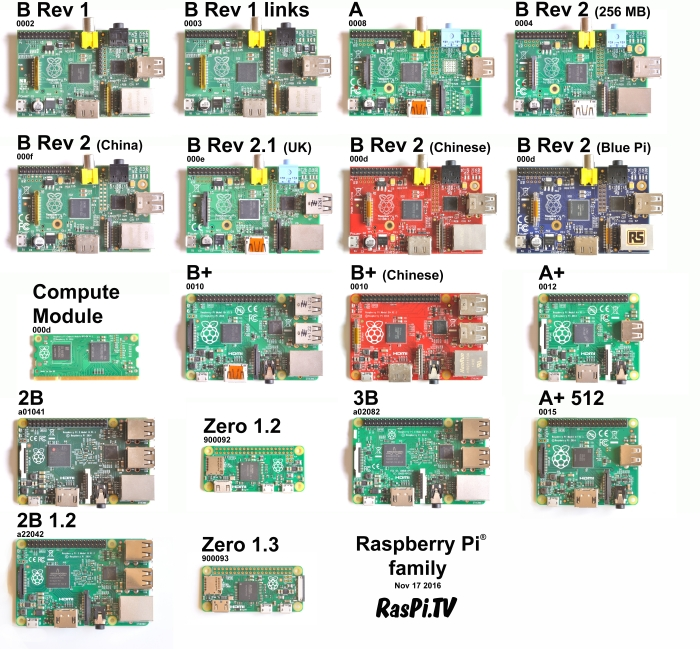
\includegraphics{images/pi-family}
	\caption{Les différents modèles de Pi}
	\label{img_family}
\end{figure}
\end{center}

\end{frame}

\section{Les caractéristiques du Pi 3}

\begin{frame}
\frametitle{Le Raspberry Pi 3}

Broadcomm est censé avoir libéré toutes les spécifications des circuits depuis 2014.

Le CPU est de la famille ARMv8 et est donc un processeur RISC. Vous retrouverez des ARM un peu partout maintenant puisque c'est le processeur le plus fréquent pour les smartphones, tablettes et autres joujous. Celui du Raspberry Pi 3 a quatre coeurs Cortex A53.

Il est 64 bits et compatible 32 bits. Toutefois il est bridé pour l'instant car le support 64 bits n'est apparu que dans une des dernières versions du kernel Linux. Pour l'instant avec la Raspbian, il est encore bridé en 32 bit.

\end{frame}

\begin{frame}
\frametitle{Le Raspberry Pi 3}

Le GPU est quant à lui un VideoCore IV double coeur. Il est compatible OpenGL et supporte l'accélération matérielle~: certains calculs 2D peuvent être déportés sur le GPU par le CPU.

Il possède un accélération matérielle pour ce qui est codé en H.264. Il supporte aussi le MPEG-2 et le VC-1 mais pour les utiliser il faut acheter une licence. Licence qui est associée au numéro de processeur du Pi.
\end{frame}

\begin{frame}
\frametitle{Le Raspberry Pi 3}
Un composant spécifique gère à la fois le LAN et l'USB ce qui peut éventuellement générer un engorgement.

Les composant WiFi et Bluetooth sont pratiques mais ils n'ont une portée que d'une dizaine de mètres contrairement aux clefs USB qui ont une portée plus proche des 30m pour le WiFi.
\end{frame}

\begin{frame}
\frametitle{Le Raspberry Pi 3}

Un détail qui a son importance, le Raspberry Pi n'a pas d'horloge interne. Elle se mets à l'heure grâce à un serveur sur Internet. C'est utile de le savoir pour certaines applications.

Pour une somme modique des horloges internes sont disponibles à brancher sur le port GPIO.

\end{frame}

%\section{Formatage et écriture de la carte SD}

\subsection{Téléchargement de l'image}

\begin{frame}
\frametitle{Où télécharger les images ?}

Les différentes images proposées par la Raspberry Pi Foundation sont à cette adresse \href{https://www.raspberrypi.org/downloads/}{https://www.raspberrypi.org/downloads/}.
\end{frame}

\begin{frame}[containsverbatim]
\frametitle{Où les télécharger ?}

Différents systèmes d'exploitation sont disponibles~:
\begin{itemize}
	\item NOOBS
	\item Raspbian
	\item Ubuntu Mate
	\item Snappy Ubuntu Core
	\item Windows 10
	\item \dots
\end{itemize}
\end{frame}

\begin{frame}[containsverbatim]
\frametitle{NOOBS}

NOOBS, \emph{New Out The Box Software} développé spécifiquement pour le Pi par la Rapsberry Pi Foundation. NOOBS n'est pas vraiment un système d'exploitation mais un gestionnaire de systèmes qui va simplifier l'installation de l'OS désiré mais également permettre le multiboot entre plusieurs systèmes présents sur la même carte SD. Solution idéale pour débuter ou pour tester les différents systèmes
existants.

\end{frame}



\begin{frame}[containsverbatim]
\frametitle{Téléchargement de l'image}

Les images sont disponibles sous forme de fichiers compressés au format zip. Pour télécharger l'image :
\begin{verbatim}
wget https://downloads.raspberrypi.org/raspbian_lite_latest
\end{verbatim}

\end{frame}

\begin{frame}[containsverbatim]
\frametitle{Vérification de l'image}
La première étape consiste à vérifier qu'il n'y a pas eu de problème lors du téléchargement en vérifiant la somme de contrôle (SHA-1).

Après téléchargement, il suffit de taper~:
\begin{verbatim}
$sha1sum 2016-11-25-raspbian-jessie-lite.zip 
6741a30d674d39246302a791f1b7b2b0c50ef9b7  2016-11-25-raspbian-jessie-lite.zip
\end{verbatim}

Il suffit de comparer alors le checksum du 	site web à celui affiché dans la console.
\end{frame}

\begin{frame}[containsverbatim]
\frametitle{Décompresser l'image}
Pour décompresser l'image, il suffit de faire~: 

\begin{verbatim}
$unzip 2016-09-23-raspbian-jessie-lite.zip
\end{verbatim}

\end{frame}

\begin{frame}[containsverbatim]
\frametitle{\'Ecriture de l'image}
Pour écrire l'image, vous pouvez toujours vous aider de l'\href{https://www.raspberrypi.org/documentation/installation/installing-images/linux.md}{aide pour Linux}.

Les images représentent les données brutes à écrire sur une carte SD. Le format \og~img~\fg est aussi valable pour faire une image disque, etc.

L'utilitaire pour écrire  cette image est \emph{dd}.
\end{frame}

\begin{frame}[containsverbatim]
\frametitle{\'Ecriture de l'image}

Il y a trois arguments pour \emph{dd}~:
\begin{description}
	\item[bs] ou block-size. C'est la taille des blocs que va écrire l'utilitaire
	\item[if] (input file) c'est la source. 
	\item[of] (output file) c'est la destination. 
\end{description}
\end{frame}

\begin{frame}[containsverbatim]
L'opération d'écriture sur un disque est irréversible. Il faut être donc absolument sûr d'écrire sur le bon disque.

Pour ceux qui sont frileux et pour les Windowsien, il y a le logiciel \href{https://etcher.io/}{Echter}.

\end{frame}

\begin{frame}[containsverbatim]
\frametitle{\'Ecriture de l'image}

Pour repérer le disque à écrire, la première possibilité est d'insérer la carte et de taper juste après la commande \emph{dmesg}~:

\begin{verbatim}
[ 6516.764148] sd 5:0:0:0: [sdb] 62333952 512-byte logical blocks: (31.9 GB/29.7 GiB)
[ 6516.765711] sd 5:0:0:0: [sdb] Write Protect is off
[ 6516.765713] sd 5:0:0:0: [sdb] Mode Sense: 03 00 00 00
[ 6516.767313] sd 5:0:0:0: [sdb] No Caching mode page found
...
\end{verbatim}

\end{frame}

\begin{frame}[containsverbatim]
\frametitle{\'Ecriture de l'image}

Sur ce listing, on voit que la carte SD a comme nom de périphérique assigné \emph{/dev/sdb}.

Pour vérifier que c'est ça, il faut utiliser \emph{fdisk}~:
\begin{verbatim}
$sudo fdisk /dev/sdb
\end{verbatim}

Puis appuyer sur \emph{p} (pour print, m pour l'aide).
\end{frame}

\begin{frame}[containsverbatim]
\frametitle{\'Ecriture de l'image}

Vous allez avoir quelque chose comme ça~:
\begin{verbatim}
Disque /dev/sdb : 29,7 GiB, 31914983424 octets, 62333952 secteurs
Unités : sectors of 1 * 512 = 512 octets
...
Périphérique Amorçage Start      Fin Secteurs  Size Id Type
/dev/sdb1              2048 62332927 62330880 29,7G  b W95 FAT32
\end{verbatim}

\end{frame}

\begin{frame}[containsverbatim]
\frametitle{\'Ecriture de l'image}

On voit que la carte fait environ 30Go avec une partition formatée en fat32, c'est typiquement une carte quand vous la sortez de la boite\dots 

Vous pouvez aussi utiliser \emph{blkid} qui est moins informatif ou bien, si la partition est montée \emph{df -h}.
\end{frame}

\begin{frame}[containsverbatim]
\frametitle{\'Ecriture de l'image}

L'image une fois écrite ne remplit pas la carte... généralement. Sur la carte après écriture, il y a trois partitions~:
\begin{enumerate}
 \item une partition FAT32 (Windows/Linux) qui contient les fichiers de démarrage de la Pi
 \item une partition ext4 (Linux) qui contient tous les fichiers de la distribution Raspbian
 \item une zone vide non partitionnée et  non formatée
 \end{enumerate}
  
\end{frame}
%\section{Personnalisation de la carte avant le gravage}

\subsection{Activer SSH}

Maintenant pour des raisons de sécurité, sur Raspbian, SSH est désactivé par défaut. Ceci pour éviter, à cause des gens qui ne modifient pas les mots de passe par défaut, que les Pi ne constituent un réservoir de bots.

\href{http://www.framboise314.fr/une-mise-a-jour-de-securite-pour-raspbian/}{http://www.framboise314.fr/une-mise-a-jour-de-securite-pour-raspbian/}


\href{https://www.raspberrypi.org/blog/a-security-update-for-raspbian-pixel/}{https://www.raspberrypi.org/blog/a-security-update-for-raspbian-pixel/}

Pour activer le SSH, il faut créer un fichier s'appelant ``ssh'' dans la partition fat32 de démarrage ou passer par ``raspi-config'' en utilisant un clavier et un écran.

Sous Linux, rien de plus simple, il suffit de faire:
\begin{verbatim}
touch /media/pascal/boot/ssh
\end{verbatim}

\subsection{\'Edition des paramètres réseaux}

Une fois branchée la Pi va récupérer une adresse IP auprès du serveur DHCP du réseau. Le plus souvent c'est votre box internet.

Il vous faudra donc regarder les logs (ou l'interface) de votre serveur DHCP (généralement votre box internet) pour voir quel IP à été attribué à la Pi pour réussir à vous connecter.

Si vous êtes sous Linux, vous pouvez trouver le Pi en scannant le réseau à la recherche des ordinateurs avec un serveur SSH accessible~:
\begin{verbatim}
nmap -p 22 192.168.0.0/16
\end{verbatim}


Sous Linux, vous avez la possibilité de fixer l'IPavant le démarrage, il suffit de faire~:
\begin{verbatim}
cd ~
mkdir pi
sudo mount /dev/sdb2 pi
\end{verbatim}

Ensuite le fichier \emph{/home/pascal/pi/etc/network/interfaces} est à éditer pour le personnaliser et donc donner une adresse fixe au Pi.

On retrouve les noms d'interface de debian, assez simples, pour les interfaces réseaux~: 
\begin{itemize}
	\item eth0 pour le LAN
	\item wlan0 pour le wifi que ce soit pour le Raspberry Pi 3 ou une clef Wifi additionnelle sur une Raspberry plus ancienne.
\end{itemize}

Sur une Raspberry Pi 3 si vous rajoutez une clef USB WiFi, vous aurez un wlan0 et un wlan1 qui sont normalement la carte interne et la clef USB respectivement.

Dans le fichier ``interfaces'', on remplace la ligne de ``eth0'' par ce contenu~:
\begin{verbatim}
allow-hotplug eth0
iface eth0 inet static
address 192.168.0.40
netmask 255.255.255.0
gateway 192.168.0.1
\end{verbatim}

Idem pour le WiFi avec une modification pour accéder aux identifiants et mots de passe du réseau WiFi auquel on se connecte~:
\begin{verbatim}
allow-hotplug wlan0
iface wlan0 inet static
address 192.168.0.41
netmask 255.255.255.0
gateway 192.168.0.1
wpa-roam /etc/wpa_supplicant/wpa_supplicant.conf
\end{verbatim}

Attention au cours de ces manipulations, il faut ne pas se tromper entre votre machine (\emph{/etc/network/interfaces}) et le Pi (\emph{/home/pascal/pi/etc/network/interfaces}). Sinon c'est un peu la catastrophe ;)

Et le fichier de configuration ``wpa\_supplicant.conf'' est à modifier selon la configuration de votre réseau sans fil~:

\begin{verbatim}
ctrl_interface=DIR=/var/run/wpa_supplicant GROUP=netdev
update_config=1

# à adapter selon la configuration de votre réseau
network={
    ssid="freebox_AERFTRE"		
    proto=WPA RSN				
    key_mgmt=WPA-PSK			
    psk="maphrasedepasse"		
}
\end{verbatim}

Par la suite si vous voulez que l'IP ne soit pas fixée par la Pi, vous pourrez le remettre en automatique et fixer un bail DHCP en récupérant l'(es) adresse(s) MAC de la Raspberry Pi.

\begin{verbatim}
iface eth0 inet dhcp

ou pour wlan0

allow-hotplug wlan0
iface wlan0 inet static
wpa-roam /etc/wpa_supplicant/wpa_supplicant.conf
iface default inet dhcp
\end{verbatim}

\begin{verbatim}
$ifconfig
eth0      Link encap:Ethernet  HWaddr b8:27:eb:1a:34:64  
          inet adr:192.168.0.50  Bcast:192.168.0.255  Masque:255.255.255.0
          adr inet6: fe80::ba27:ebff:fe1a:4048/64 Scope:Lien
          UP BROADCAST RUNNING MULTICAST  MTU:1500  Metric:1
          RX packets:3630835 errors:0 dropped:13 overruns:0 frame:0
          TX packets:3365928 errors:0 dropped:0 overruns:0 carrier:0
          collisions:0 lg file transmission:1000 
          RX bytes:2510486112 (2.3 GiB)  TX bytes:2571670733 (2.3 GiB)

lo        Link encap:Boucle locale  
          inet adr:127.0.0.1  Masque:255.0.0.0
          adr inet6: ::1/128 Scope:Hôte
          UP LOOPBACK RUNNING  MTU:65536  Metric:1
          RX packets:284 errors:0 dropped:0 overruns:0 frame:0
          TX packets:284 errors:0 dropped:0 overruns:0 carrier:0
          collisions:0 lg file transmission:1 
          RX bytes:28401 (27.7 KiB)  TX bytes:28401 (27.7 KiB)

wlan0     Link encap:Ethernet  HWaddr 74:da:38:1a:b4:b8  
          UP BROADCAST MULTICAST  MTU:1500  Metric:1
          RX packets:0 errors:0 dropped:2 overruns:0 frame:0
          TX packets:0 errors:0 dropped:0 overruns:0 carrier:0
          collisions:0 lg file transmission:1000 
          RX bytes:0 (0.0 B)  TX bytes:0 (0.0 B)
\end{verbatim}

Par exemple ici l'adresse MAC pour eth0 est b8:27:eb:1a:34:64 et pour wlan0 l'adresse MAC est 74:da:38:1a:b4:b8.

\subsection{Ajout d'un partition /home}

Le plus simple est d'utiliser gparted ou parted. Ceci est à faire avant l'écriture de la carte depusi un ordinateur GNU/Linux.

Ici la carte est le péripherique ``sdb'' mais vous devez le remplacer par l'identifiant de votre disque. 

Avec parted en ligne de commande, on va agrandir un peu la partition système~:
\begin{verbatim}
$parted /dev/sdb
$print

Modèle: Generic USB SD Reader (scsi)
Disque /dev/sdb : 31,9GB
Taille des secteurs (logiques/physiques): 512B/512B
Table de partitions : msdos
Disk Flags: 

Numéro  Début   Fin     Taille  Type     Système de fichiers  Fanions
 1      4194kB  70,3MB  66,1MB  primary  fat16                lba
 2      70,3MB  1390MB  1320MB  primary  ext4

$resizepart 2
$2000MB
$print

Modèle: Generic USB SD Reader (scsi)
Disque /dev/sdb : 31,9GB
Taille des secteurs (logiques/physiques): 512B/512B
Table de partitions : msdos
Disk Flags: 

Numéro  Début   Fin     Taille  Type     Système de fichiers  Fanions
 1      4194kB  70,3MB  66,1MB  primary  fat16                lba
 2      70,3MB  2000MB  1930MB  primary  ext4
\end{verbatim}

Pour ajouter la partition ``/home''~:

\begin{verbatim}
$mkpart
$primaire
$ext4
$2001MB
$31900MB
$print

Modèle: Generic USB SD Reader (scsi)
Disque /dev/sdb : 31,9GB
Taille des secteurs (logiques/physiques): 512B/512B
Table de partitions : msdos
Disk Flags: 

Numéro  Début   Fin     Taille  Type     Système de fichiers  Fanions
 1      4194kB  70,3MB  66,1MB  primary  fat16                lba
 2      70,3MB  2000MB  1930MB  primary  ext4
 3      2001MB  31,9GB  29,9GB  primary  ext4                 lba

$quit

$sudo mkfs.ext4 /dev/sdb3

\end{verbatim}

Ensuite il faut éditer le fichier `/etc/fstab' sur la carte.

\begin{verbatim}
proc                           /proc    proc    defaults                  0       0
/dev/mmcblk0p1  /boot    vfat    defaults                   0       2
/dev/mmcblk0p2  /             ext4    defaults,noatime 0       1
/dev/mmcblk0p3  /home ext4    defaults,noatime  0       1
\end{verbatim}

Enfin il faut copier le contenu du ``home'' de la pi sur la nouvelle partition~:

\begin{verbatim}
$cd /media/pascal/0aed834e-8c8f-412d-a276-a265dc676112/home/
$sudo cp -Ra * /media/pascal/f59b2c6c-b34c-45ec-b945-e01823d08bf5/
\end{verbatim}

\subsection{Préserver la carte SD}

\subsubsection{Mettre la carte SD en lecture seule}
Certains, pour augmenter la durée de vie de la carte SD, monte la racine sur la clef en lecture seule. Ceci pour éviter les écritures des logs et autres qui sont fréquents et qui ``abiment'' la carte SD. 

Avec la diminution du prix des cartes SD, cela devient moins nécessaire. D'expérience une carte SD utilisée sur un Pi peut tenir plusieurs années. En outre cela a un grave inconvénient si on utilise le Pi comme routeur ou comme serveur c'est qu'on perd les logs qui sont stockés en mémoire vive. Et les logs, c'est plutôt utile\dots

Un moyen de contourner serait d'écrire les logs sur une clef usb mais ça a grosso modo la même durée de vie qu'une carte SD (voire moins). Le mieux est surement de prendre une carte minimum genre 8Go qui n'est pas trop chère.

La manipulation pour passer la carte en lecture seule est décrite ci-dessous. 

Tout d'abord il faut mettre en mémoire vive les fichiers d'ajustement du temps (la Raspberry n'a pas d'horloge interne).

\begin{verbatim}
$sudo ln -s /var/run/adjtime /etc/adjtime
$sudo nano +61 /etc/init.d/hwclock.sh
\end{verbatim}

Dans le fichier qui vient d'ouvrir à la ligne  61, il faut changer le -f (vrai si le fichier existe et est un fichier régulier) en -L (vrai si le fichier existe et est un lien symbolique).

Ce qui donne~:
\begin{verbatim}
if [ -w /etc ] && [ ! -L /etc/adjtime ] && [ ! -e /etc/adjtime ]; then
\end{verbatim}

Puis on crée un fichier cache dans ``/etc/blkid/blkid.tab''. Nous allons le déplacer sur un ramdisk.

\begin{verbatim}
$sudo nano /etc/environment
$BLKID_FILE="/var/run/blkid.tab"
\end{verbatim}

Il faut éditer le fichier ``/etc/fstab''~:

\begin{verbatim}
proc				/proc	proc    defaults							0	0
tmpfs			/tmp	tmpfs nodev,nosuid,size=30M,mode=1777		0	0
tmpfs			/var/log	tmpfs nodev,nosuid,size=30M,mode=1777		0	0
/dev/mmcblk0p1  	/boot      	vfat    defaults,noatime,ro          				0       2
/dev/mmcblk0p2  	/               	ext4    defaults,noatime,ro,errors=remout-ro 	0       1
\end{verbatim}

Puis il faut dans le fichier ``/etc/default/rcS'' changer la valeur de RAMTMP~:

\begin{verbatim}
$sudo nano /etc/default/rcS
RAMTMP=yes
\end{verbatim}

Enfin dans ``/etc/profile''~:
\begin{verbatim}
mount | grep ' on / ' | grep '(ro' && echo "Montage en lecture-écriture" && 
sudo mount -o remount,rw /
\end{verbatim}

Et on reboote.

\subsubsection{Ajuster les paramètres pour préserver la carte SD}

Pour ménager la chèvre et le chou, on utilise les recommandations faites pour préserver les lecteurs SSD sur les PCs fixes.

Dans le fichier ``/etc/fstab'', on change quelques petites choses~:

\begin{verbatim}
proc				/proc proc 	defaults						       0  0
tmpfs			/tmp  tmpfs	nodev,nosuid,size=30M,mode=1777  0  0
/dev/mmcblk0p1  	/boot vfat    	defaults,noatime          			        0  2
/dev/mmcblk0p2  	/          ext4    	defaults,noatime,errors=remout-ro    0  1
\end{verbatim}

L'argument ``noatime'' est un moyen de supprimer l'écriture de la date de la dernière lecture ce qui minimise les écritures sur le disque.

De plus un crée on crée une partition en mémoire pour /var/tmp dans lequel le système écrit beaucoup.

Puis il faut dans le fichier ``/etc/default/rcS'' changer la valeur de RAMTP~:

\begin{verbatim}
$sudo nano /etc/default/rcS
RAMTMP=yes
\end{verbatim}

Pour que les changements prennent effet, redémarrez votre Pi.
%\section{Démarrage}

\begin{frame}[containsverbatim]
\frametitle{Démarrage}

\begin{enumerate}
	\item il va chercher un premier fichier bootcode sur la partition FAT32 qui est exécuté par le GPU
	\item il va chercher un second fichier start\_elf sur la partition FAT32 qui est exécuté par le GPU
	\item le GPU va sonner le CPU pour qu'il démarre en passant le noyau avec les arguments qui vont bien
	\item Le CPU se lance avec le kernel (noyau) et le démarrage devient celui de Linux~:
		\begin{itemize}
			\item chargement en mémoire du kernel
			\item montage en lecture de la partition /
			\item ...
		\end{itemize}
\end{enumerate}

\end{frame}

\begin{frame}[containsverbatim]
\frametitle{Démarrage}

Le démarrage se fait à l'aide du GPU et non du CPU.

Les fichiers de démarrage du GPU \emph{bootcode} et \emph{start\_elf} sont propriétaires et sont distribués sous la forme de binaire.

Le démarrage ne se fait pas avec les outils GNU/Linux habituel : \emph{grub} ou \emph{lilo} comme sur un PC normal. Le démarrage va dépendre de la présence de cette fameuse partition fat32 au début de la carte. 

\end{frame}

\begin{frame}[containsverbatim]
\frametitle{Démarrage}
Le fichier important sur un Raspberry est le fichier ``config.txt''. En effet ce fichier est utilisé pour personnaliser le démarrage du Pi en ajoutant la caméra, modifier la mémoire réservé au gpu, ... On y trouve aussi plein de paramètres pour configurer la sortie HDMI si vous lancez le Pi avec une interface graphique.

\end{frame}

\begin{frame}[containsverbatim]
\frametitle{Gestion de la mémoire}

La mémoire d'un Raspberry est commune entre le GPU et le CPU. Selon l'usage que vous faites du Raspberry, par exemple utiliser ou non la caméra ou l'utiliser comme centre multimédia, il peut être intéressant de modifier la quantité de mémoire allouée au GPU. 

Le minimum pour le GPU est 16Mo. Il est nécessaire d'avoir 64Mo pour utiliser la caméra qui est aussi la valeur par défaut~:
\begin{verbatim}
gpu_mem=16
\end{verbatim} 
Ici on règle la mémoire à 16Mo
\end{frame}


\begin{frame}[containsverbatim]
\frametitle{Gestion de la mémoire}
Les valeurs maximales pour la mémoire attribuée au GPU sont quant à elles de 448Mo pour 512Mo de mémoire et 944Mo pour 1024Mo de mémoire.

Il y a aussi la possibilité de définir la mémoire en fonction de la taille mémoire installée sur le Pi. La spécification de la mémoire en fonction de la taille mémoire installée écrase le paramètre fixé par ``gpu\_mem''.

\begin{verbatim}
gpu_mem_1024=64
gpu_mem_512=32
gpu_mem_256=16
\end{verbatim}
\end{frame}

\begin{frame}[containsverbatim]
\frametitle{Gestion de la mémoire}

Ici on fixe 64Mo pour une mémoire de 1Go (Raspberry Pi 3), 32Mo pour une Raspberry Pi2+, ... Ces paramètres sont utiles si vous personnalisez une carte pour l'installer sur différents Pi.

Les paramètres de ``config.txt'' pour la plupart ne sont pas nécessairement à taper à la main dans le fichier. En effet l'utilitaire ``raspi-config'' permet d'éditer le fichier via un menu plus convivial.

\end{frame}
%\section{Connexion SSH à la Pi}

Pour se connecter à la Pi, il faut que la Pi et l'ordinateur soient connectés tous les deux sur ethernet et que la Pi soit accessible depuis l'ordinateur (pas de routeur ou de pare-feu entre les deux par exemple). 

\subsection{Se connecter à la Pi}

Pour se connecter il suffit de taper~:
\begin{verbatim}
$ssh 192.168.0.56 -l pi
$raspberry (c'est le mot de passe par défaut)

The authenticity of host '192.168.0.56 (192.168.0.56)' can't be established.
ECDSA key fingerprint is SHA256:jxN8A+IwAD+axlznp4wLME8Tpi36yCVW8duJmvA0yfs.
Are you sure you want to continue connecting (yes/no)? 

$yes

Warning: Permanently added '192.168.0.56' (ECDSA) to the list of known hosts.
\end{verbatim}

Les Pis lors du premier démarrage créent une clef unique pour le serveur, il n'y a donc pas besoin de régénérer les clefs pour le serveur SSH.

\subsection{Créer une clef pour la connexion sans mot de passe}

Vous pouvez le faire sur votre poste linux, utiliser putty-keygen ou le faire dans la pi.

Pour générer un clef si vous n'en avez pas déjà, il faut utiliser ``ssh-keygen''

\begin{verbatim}
$ssh-keygen
Generating public/private rsa key pair.
Enter file in which to save the key (/home/pi/.ssh/id_rsa): 
$ (entrée) par défaut
Created directory '/home/pi/.ssh'.
Enter passphrase (empty for no passphrase): 
$ (taper un mot de passe, vide pour pas de mot de passe)
Enter same passphrase again: 
$ (confirmer le mot de passe)
Your identification has been saved in /home/pi/.ssh/id_rsa.
Your public key has been saved in /home/pi/.ssh/id_rsa.pub.
The key fingerprint is:
31:96:37:e1:0d:93:95:a2:51:ff:80:1a:79:be:bb:ad pi@raspberrypi
The key's randomart image is:
+---[RSA 2048]----+
|         .=o..   |
|        .+oB.    |
|        Bo*.+    |
|       ..O . o   |
|        S .   .  |
|           .     |
|          .      |
|           o     |
|          Eo.    |
+-----------------+
\end{verbatim}

Pour activer la connexion par clef, il suffit de quelques modifications~:
\begin{verbatim}
$mv .ssh/id_rsa.pub .ssh/authorized_keys
$vi .ssh/id_rsa
(copier la clef privée dans un fichier ``clef_raspberry'' du répertoire .ssh
de votre ordinateur)
$rm .ssh/id_rsa
\end{verbatim}

Renommer le fichier ``id\_rsa.pub'' en ``authorized\_keys'' permet notamment au serveur de reconnaître que l'ordinateur avec la clef privé correspondante (id\_rsa) est autorisée à se connecter  sur la Pi avec ce compte.

Il faut donc bien copier ``id\_rsa'' sous ce nom ou un autre dans votre compte personnel et dans le répertoire .ssh pour un ordinateur GNU/Linux ou Mac OS.

Avec putty sous Windows vous trouverez de l'aide à cette \href{https://www.howtoforge.com/ssh_key_based_logins_putty}{page}.  

Sous GNU/Linux (et Mac OS), après il suffit de configurer ou de créer le fichier ``.ssh/config'~:

\begin{verbatim}
Host monpi
    Hostname 192.169.0.56
    User pi
    Port 22
    IdentityFile clef_raspberry
\end{verbatim}

Vous pourrez vous connecter sans mot de passe simplement en tapant ``ssh monpi''.

%\section{Les utilitaires de configuration de la Pi}



\begin{frame}[containsverbatim]
\frametitle{Utilitaires}
Pour simplifier les choses pour les débutants, les concepteurs de la Raspbian ont inclus deux utilitaires spécifique à la Pi dans la distribution.

Le premier outil est \emph{raspi-config}. C'est un utilitaire clique-bouton (NCURSES en mode console) pour accéder à des fonctions spécifiques de la Pi ou pour lancer des commandes Linux.

L'autre outil est \emph{rpi-update} qui permet de mettre à jour le firmware de la Pi. Il est à lancer régulièrement pour avoir son système à jour. Ce qui est différent des mises à jour de Raspbian.

\end{frame}

\subsection{raspi-config}

\begin{frame}[containsverbatim]
\frametitle{raspi-config}

Quand vous lancez un Rapsberry Pi, il est important de faire quelques réglages~:
\begin{enumerate}
	\item Changer le mot de passe
	\item Internationalization Options, changer les locales (fr\_FR.UTF-8 UTF-8)
	\item Internationalization Options, changer le timezone (Paris)
\end{enumerate}

\end{frame}

\begin{frame}[containsverbatim]
\frametitle{raspi-config}

Toutes ces commandes sont en fait des commandes debian mais elle sont plus simples à utiliser dans ``raspi-config''.

Parmi les autres options, il y a l'activation de la caméra et dans les options avancées, il y a également des choses intéressantes~:
\begin{description}
	\item[Hostname] Changer l'Hostname pour y accéder par ce nom plutôt que par l'ip
	\item[Memory Split] la mémoire allouée au GPU
	\item[SPI] utile pour activer la compatibilité avec des hat comme PiFace
	\item[\dots]
\end{description}
\end{frame}

\subsection{rpi-update}

\begin{frame}[containsverbatim]
\frametitle{rpi-update}

Cet outil est lié au Raspberry, c'est pour récupérer et mettre à jour le firmware.

En plus des paquets, il est important de maintenir à jour son Pi y compris son firmware. Il faut éviter absolument de couper l'alimentation ou de couper la connexion SSH pendant la mise à jour du firmware.

La commande est très simple~:

\begin{verbatim}
$rpi-update
\end{verbatim}

\end{frame}

%\section{Sécurisation de votre Raspberry Pi}

\subsection{Changer le mot de passe}

La première étape est de changer le mot de passe par défaut. Il suffit de se connecter et de faire~:
\begin{verbatim}
passwd
\end{verbatim}

Choisissez un mot de passe le plus sécuritaire possible. 

Vous pouvez aussi créer un utilisateur spécifique. Par exemple pour ajouter un utilisateur \emph{pascal}~:
\begin{verbatim}
$sudo adduser pascal
....
\end{verbatim}

Il faut veiller si vous bricolez avec votre pi de lui donner les mêmes droits que l'utilisateur pi. Pour cela, il faut éditer le fichier \emph{/etc/groups}.

Ce sont surtout le groupe \emph{sudo}, \emph{SPI} qui sont utiles car ils permettront de lancer des commandes en tant que \emph{root} et d'avoir le contrôle sur les interfaces de la pi.

Avec le nouvel utilisateur ``username'', vous devez écrire la commande suivante pour avoir la même configuration que l'utilisateur ``Pi'' (le tout sur une même ligne)

\begin{verbatim}
$sudo usermod -a -G adm,dialout,cdrom,sudo,audio,video,
plugdev,games,users,input,netdev,spi,i2c,gpio  username
\end{verbatim}

Si vous voulez supprimer le compte pi par sécurité, il suffit de faire~:
\begin{verbatim}
$sudo deluser pi
\end{verbatim}

\subsection{Pare-feu}

Vous devez mettre un pare-feu. Surtout si vous utilisez le Pi comme serveur et donc qui est ``face'' à internet. 

Attention, quelque soit le pare-feu, il faut laisser le port 22 ouvert pour vous connecter avec SSH sinon votre Raspberry Pi deviendra une brique... Il faut ouvrir le port et lancer le pare-feu au cours d'une session SSH et se connecter dans une nouvelle connexion pour vérifier que le port est bien ouvert !

Avant tout il est utile de sauvegarder un pare-feu vide au cas où les choses tournent mal.

\begin{verbatim}
$sudo iptables-save  ~/iptables.empty
\end{verbatim}

Vous pouvez faire un pare-feu simple ``à la main'' avec \emph{iptables}~:
\begin{verbatim}
#!/bin/sh

IPTABLES=/sbin/iptables

# Creation des tables
$IPTABLES -N TCP
$IPTABLES -N UDP

# Politique par défaut
$IPTABLES -P FORWARD DROP
$IPTABLES -P OUTPUT ACCEPT
$IPTABLES -P INPUT DROP

# Laisser passer les connexions existantes ou provenant du loop
$IPTABLES -A INPUT -m conntrack --ctstate RELATED,ESTABLISHED -j ACCEPT
$IPTABLES -A INPUT -i lo -j ACCEPT

# Bloquer les invalides
$IPTABLES -A INPUT -m conntrack --ctstate INVALID -j DROP

# Misc
$IPTABLES -A INPUT -p icmp --icmp-type 8 -m conntrack --ctstate NEW -j ACCEPT
$IPTABLES -A INPUT -p udp -m conntrack --ctstate NEW -j UDP
$IPTABLES -A INPUT -p tcp --syn -m conntrack --ctstate NEW -j TCP
$IPTABLES -A INPUT -p udp -j REJECT --reject-with icmp-port-unreachable
$IPTABLES -A INPUT -p tcp -j REJECT --reject-with tcp-reset
$IPTABLES -A INPUT -j REJECT --reject-with icmp-proto-unreachable

# Ouvrir le port 22 pour SSH
$IPTABLES -A TCP -p tcp --dport 22 -j ACCEPT

...
\end{verbatim}

En cas de problème, utiliser le fichier qui permet de restaurer un pare-feu vide~:

\begin{verbatim}
sudo iptables-restore ~/iptables.empty
\end{verbatim}

Attention tous les fichiers du firewall doivent être accessibles seulement par le root.

\begin{verbatim}
$sudo chmod 700 02-firewall
$sudo chown root:root 02-firewall
\end{verbatim}

Le fichier du firewall est à mettre dans le répertoire ``/etc/network/if-pre-up.d''. Il sera exécuter dès que le réseau va devenir accessible. Vous pouvez aussi le placer en fin de lancement de Linux~: dans le fichier ``/etc/rc.local''.

Sinon il y a un paquet très efficace et pratique~: \emph{arno-iptables-firewall}. C'est un script BASH qui fait un pare-feu de bonne facture. Il faut indiquer les ports à laisser ouvert lors de l'installation. Il gère aussi des règles plus complexes~: NAT, DMZ, ports ouverts sur le LAN et pas sur internet, ... Le fichier de configuration est assez simple et assez didactique.

Pour l'installer, c'est comme pour n'importe quel paquet Debian~:
\begin{verbatim}
$sudo apt-get install arno-iptables-firewall
\end{verbatim}

Lors de l'installation, il vous pose les questions suivantes~:
\begin{enumerate}
	\item Faut-il gérer automatiquement le pare-feu. La réponse est oui.
	\item Les interfaces réseaux externes sont les interfaces réseaux qui seront filtrées par le pare-feu. Pour être le plus sécuritaire il vaut mieux toutes les ajouter en mettant~: eth+ wlan+
	\item Il demande si le DHCP est autorisé sur les réseaux externes. Si vous avez ajouter toutes les interfaces répondez oui. Si vous n'avez pas mis votre réseau local en interface externe vous pouvez répondre non.
	\item Ports TCP ouverts. Il y en a un à rajouter absolument c'est le port 22 (du SSH) pour se connecter au Pi. Après vous pourrez en rajouter à loisir au fil de votre configuration.
	\item Ports UDP ouverts. normalement il y en a pas sauf si vous installez un serveur OpenVPN par exemple.
	\item Faut-il autoriser les ping\dots Si vous n'installez pas OpenVPN il vaut mieux répondre non. 
	\item Interfaces réseaux ethernes. CE sont les interfaces réseaux qui ne seront pas protégées. Par défaut c'est vide (cf 2.).
	\item Faut-il redémarrer le pare-feu. Oui
\end{enumerate}

Pour stopper le pare-feu, relancer et lancer le pare-feu les commandes sont respectivement~:
\begin{verbatim}
$sudo service arno-iptables-firewall stop
$sudo service arno-iptables-firewall restart
$sudo service arno-iptables-firewall start
\end{verbatim}

Pour le reconfigurer vous avez deux possibilités. Soit utiliser l'interface NCURSES en mode console en faisant~:
\begin{verbatim}
$sudo dpkg-reconfigure arno-iptables-firewall
\end{verbatim}

Soit en éditant le fichier ``/etc/arno-iptables-firewall/conf.d/00debconf.conf'' directement.

Il y a des réglages beaucoup plus avancés disponibles dans le fichier firewall.conf du répertoire ``/etc/arno-iptables-firewall''.

\subsection{Mise à jour}

Il faut maintenir votre Raspberry Pi à jour... Pour tout ce qui est fourni par les paquets Debian, il suffit de faire de temps en temps un petit~:
\begin{verbatim}
$sudo apt-get update
$sudo apt-get upgrade -y
$sudo apt-get dist-upgrade -y
\end{verbatim}

Si la mise à jour contient une mise à jour du noyau, il faudra redémarrer le Pi.

Comme vu précédemment il y a aussi le firmware à mettre à jour avec la commande spéciale~:
\begin{verbatim}
$sudo rpi-update
\end{verbatim}

Le mieux est de créer un alias dans le fichier \emph{.bashrc}~:
\begin{verbatim}
alias update=sudo rpi-update && sudo apt-get update && sudo apt-get upgrade -y && sudo apt-get dist-upgrade -y 
\end{verbatim}

Si vous avez installer un serveur web avec WordPress ou Yunohost il vous faudra aussi mettre à jour les composants en plus.

De temps en temps, des paquets ne sont plus nécessaires, dans ce cas il vous le signale quand vous faites des mises à jour. Il faut alors taper~:
\begin{verbatim}
$sudo apt-get autoremove
\end{verbatim}

\subsection{Bloquer les connexions SSH non basées sur les clefs}

Pour éviter les connexions qui utilisent un mot de passe au lieu de la clef privé/clef publique, il faut changer cette ligne (c'est la dernière ligne) dans ``/etc/ssh/sshd\_config''~:

\begin{verbatim}
UsePAM no
\end{verbatim}

Il faut aussi empêcher les connexions en tant que root (c'est la ligne 28)~:
\begin{verbatim}
PermitRootLogin no
\end{verbatim}

Puis il faut redémarrer le serveur~:

\begin{verbatim}
$sudo service ssh restart
\end{verbatim}



\section{Installer Privoxy}

\begin{frame}[containsverbatim]
\frametitle{Privoxy}
Privoxy est un proxy qui ne met pas en cache mais filtre le contenu des pages lues pour enlever notamment les publicités et peut également modifier les pages web.

\end{frame}

\subsection{Installation}

\begin{frame}[containsverbatim]
\frametitle{Privoxy}

Pour l'installation il suffit de faire un~:
\begin{verbatim}
$sudo apt-get install privoxy
\end{verbatim}

\end{frame}

\begin{frame}[containsverbatim]
\frametitle{Installation}

Il y a quelques réglages à faire. Tout d'abord il faut le configurer pour qu'il écoute le réseau local.

\begin{verbatim}
$sudo nano +761 /etc/privoxy/config
listen-address  192.168.0.56:8118
\end{verbatim}

\end{frame}

\begin{frame}[containsverbatim]
\frametitle{Configuration}

On va enlever le logging de privoxy pour éviter de stocker votre historique Web (bien que par défaut privoxy ne stocke que les évènements graves). Vous devez le réactiver si vous avez des problèmes de navigation pour le débogage.

\begin{verbatim}
$sudo nano +455
#logfile logfile
\end{verbatim}

\end{frame}

\begin{frame}[containsverbatim]
\frametitle{Configuration}

Pour limiter l'accès à votre réseau local (c'est mieux\dots), il suffit de faire~:
\begin{verbatim}
$sudo nano +1062
permit-access  192.168.0.0/24
\end{verbatim}

\end{frame}

\begin{frame}[containsverbatim]
\frametitle{Configuration}

On redémarre le serveur pour tenir compte des changements~:
\begin{verbatim}
$sudo service privoxy restart
\end{verbatim}

\end{frame}

\begin{frame}[containsverbatim]
\frametitle{Pare-feu}

Ensuite il y a un nouveau port ouvert, le port 8118, il faut donc modifier le firewall. Soit avec~:
\begin{verbatim}
$sudo dpkg-reconfigure arno-iptables-firewall
\end{verbatim}

\end{frame}

\begin{frame}[containsverbatim]
\frametitle{Pare-feu}

ou bien dans le fichier du firewall

\begin{verbatim}
$IPTABLES -A TCP -p tcp --dport 8118 -j ACCEPT
\end{verbatim}

\end{frame}

\begin{frame}[containsverbatim]
\frametitle{Dans le navigateur}

Ensuite il faut dans votre navigateur, régler le proxy~:
\begin{description}
	\item [Firefox] je vous conseille d'utiliser l'extension FoxyProxy qui permet de changer à la volée le proxy
	\item [Chromium] SwitchyOmega qui permet de changer à la volée le proxy
\end{description}

\end{frame}

\begin{frame}[containsverbatim]
\frametitle{Dans le navigateur}

Si vous voulez que le proxy se configure automatiquement pour les machines de votre réseau. Il faut pouvoir ajouter une ligne à la configuration de votre serveur DHCP et mettre à disposition un fichier sur le serveur web. La manipulation est expliquée \href{https://www.howtoforge.com/squid-proxy-server-on-ubuntu-9.04-server-with-dansguardian-clamav-and-wpad-proxy-auto-detection}{ici}.

\end{frame}

\subsection{Réglages des filtres}

\begin{frame}[containsverbatim]
\frametitle{Filtrage}

Les fichiers ``user.action'' et ``user.filter'' sont là que vous allez faire vos modifications.

Par exemple si vous souhaitez qu'un site ne soit pas filtré, comme \href{numerama.com}{numerama} un super site que vous voulez aider en acceptant la pub. Il faut faire~:

\begin{verbatim}
$sudo nano +158 user.action
.numerama.com
\end{verbatim}

\end{frame}

\begin{frame}[containsverbatim]
\frametitle{Filtrage}

Par défaut, les cookies sont autorisés seulement s'il s'agit de cookies de session, si vous voulez qu'un cookie à plus long terme soit conservé, il faut ajouter le site dans la partie adéquate~:
\begin{verbatim}
$sudo nano +90 user.action
.github.com
\end{verbatim}

\end{frame}

\begin{frame}[containsverbatim]
\frametitle{Filtrage}

Vous pouvez utiliser le fichier trust pour limiter les web à visiter comme par exemple limiter l'accès seulement à quelques sites, pour les enfants par exemple.

\begin{verbatim}
$sudo nano +511 config
trustfile trust
\end{verbatim}

Dans trust, vous pouvez les sites qui sont autorisés~:
\begin{verbatim}
~.starinux.org
\end{verbatim}

N'oubliez pas de relancer le serveur.

\end{frame}
\section{Installer un serveur VPN}

Le but est de créer un serveur VPN. Qu'est ce que le VPN ? C'est l'acronyme de Virtual Private Network. Il va créer un pont crypté entre deux ordinateurs et les requêtes réseaux vont être déportés sur le serveur. Toutes les requêtes réseaux du client vont sortir seulement à travers du tunnel crypté.

Son utilité ? Avoir son serveur VPN est utile par exemple quand vous êtes dans un Starbucks ou dans un hotel. Vous ne savez qui est à l'écoute sur le réseau et vos communications peuvent être interceptés. Pour éviter ce désagrément, vous activez le VPN et ainsi les communications seront cryptés et hors de portée de ceux qui écoutent. Les requêtes seront ``déplacées'' sur l'ordinateur serveur, votre Raspberry au chaud à la maison.

Il peut également être utilisé comme accès au réseau local pour permettre des réparations sur l'ordinateur d'un tiers (après avoir son accord). Ce système peut se substituer ou s'ajouter à un VNC (Virtual Network Connexion)~: en effet vous pouvez sécuriser l'accès au VNC en passant par le tunnel sécurisé du VPN.

Il est à noter que des serveurs VPN commerciaux existent. Dans ce cas vous données sont cryptées de votre ordinateur à au site du VPN commercial et après passent en clair. Le stockage de vos données de connexion varient selon les opérateurs de VPN que vous utilisez. 

Sur le Raspberry, on peut établir un réseau VPN de type PPTP qui n'est pas le protocole le plus sécurisé. Nous nous intéresserons au protocole le plus sécurisé~: le protocole OpenVPN.

La cryptage est asymétrique avec une paire clef privée et clef publique. Il y a une paire de clefs pour le serveur et une paire pour le client.

\subsection{Installation}

L'installation à la main supposerait~:
\begin{enumerate}
	\item télécharger les paquets nécessaires
	\item créer les deux paires de clefs
	\item configurer le serveur
	\item préparer le fichier client
	\item installer la connexion VPN sur le client avec le fichier client
\end{enumerate}

Pour en profiter, il faut installer git qui est un logiciel permettant de récupérer des applications à compiler (entre autres)~:
\begin{verbatim}
$sudo apt-get install git
\end{verbatim}

Fort heureusement un script disponible \href{https://github.com/Nyr/openvpn-install}{ici}, facilite ça et le rend interactif~:

\begin{verbatim}
$wget https://git.io/vpn -O openvpn-install.sh 
$sudo bash openvpn-install.sh
\end{verbatim}

Le premier renseignement demandé est l'IP du Raspberry sur le réseau interne. Pour moi 192.168.0.56.

Le second est le port par défaut. Ce n'est pas la peine de le changer.

Ensuite vous devez choisir les DNS qui seront utilisés pour que le serveur puisse résoudre les noms de domaine en sortie du VPN. Je vous conseille OpenDNS bien que OpenDNS appartienne maintenant à Oracle. Le mieux est d'utiliser les serveurs de l'\href{https://www.opennicproject.org/}{OpenNIC}.

Ensuite il vous demande le nom du fichier à créer. Ici on va laisser le nom par défaut. Si vous avez plusieurs profils il vous faudra donner un nom plus explicite.

Il vous demande de fournir l'''external IP'', c'est qu'il a remarqué que vous étiez derrière un NAT donc il demande l'adresse publique qu'il va mettre dans le fichier client pour que ce dernier puisse se connecter au serveur depuis internet. 

Enfin il vous demande le mot de passe pour vous connecter au VPN. Vous devez choisir un mot de passe fort voire très fort car la plupart des applications permettent de le garder en mémoire. 

Après le script va télécharger et installer les paquets. Il installe notamment~:
\begin{itemize}
	\item OpenVPN, qui est le programme permettant de se connecter à un VPN ou qui permet de faire un serveur VPN.
	\item Easy-RSA, sur un dépot \href{https://github.com/OpenVPN/easy-rsa}{git}, c'est le programme qui permet de créer facilement des clefs RSA pour le client et pour le serveur. 
\end{itemize}

L'étape la plus longue est la création de la clef privée du serveur qui peut parfois prendre dix minutes sur un Raspberry Pi 2 si il y a un manque d'entropie. Pour aller plus vite dans la génération de la client, vous pouvez générer de l'entropie par exemple en téléchargeant quelque chose de gros sur le réseau dans une deuxième session~:
\begin{verbatim}

\end{verbatim}



Dans le répertoire courant, un nouveau fichier ``.ovpn'' est apparu. C'est le fichier client qui servira à configurer votre portable.

\begin{verbatim}
client
dev tun
proto udp
sndbuf 0
rcvbuf 0
remote 88.190.40.134 1194
resolv-retry infinite
nobind
persist-key
persist-tun
remote-cert-tls server
cipher AES-256-CBC
comp-lzo
setenv opt block-outside-dns
key-direction 1
verb 3
...
\end{verbatim}

Dans le répertoire ``/etc/openvpn'', vous trouverez les clefs du serveur ainsi que le fichier de configuration, ``server.conf'',  auquel il faut faire des modifications.

Il faut modifier la première ligne dans ce fichier de configuration en rajoutant~:
\begin{verbatim}
local 192.168.0.56
\end{verbatim}

Ce qui donne comme fichier de configuration~:
\begin{verbatim}
local 192.168.0.56
port 1194
proto udp
dev tun
sndbuf 0
rcvbuf 0
ca ca.crt
cert server.crt
key server.key
dh dh.pem
tls-auth ta.key 0
topology subnet
server 10.8.0.0 255.255.255.0
ifconfig-pool-persist ipp.txt
push "redirect-gateway def1 bypass-dhcp"
push "dhcp-option DNS 208.67.222.222"
push "dhcp-option DNS 208.67.220.220"
keepalive 10 120
cipher AES-256-CBC
comp-lzo
user nobody
group nogroup
persist-key
persist-tun
status openvpn-status.log
verb 3
crl-verify crl.pem
\end{verbatim}

Le serveur openvpn se comporte pour ses clients comme un serveur DHCP. La ligne ``server'' indique une plage d'adresse doit être une plage d'adresse qui est \emph{absolument différente} de la plage d'adresse que vous utilisez pour votre réseau interne. 

Cette plage d'adresse contient les IPs des clients du VPN. Vous savez donc que cette plage d'adresse est le réseau ``interne'' pour le firewall. Vous avez aussi besoin de savoir que l'interface réseau créée par un VPN est ``tun0''. Vous pouvez le vérifier en tapant~:
\begin{verbatim}
$ifconfig
\end{verbatim}  

Pour ajouter les serveurs DNS de l'OpenNIC, il suffit de les choisir sur leur \href{https://www.opennicproject.org/}{page}.

On choisit par exemple 87.98.175.85 et 193.183.98.154. Cela nous donnerait comme fichier de configuration~:
\begin{verbatim}
local 192.168.0.56
port 1194
proto udp
dev tun
sndbuf 0
rcvbuf 0
ca ca.crt
cert server.crt
key server.key
dh dh.pem
tls-auth ta.key 0
topology subnet
server 10.8.0.0 255.255.255.0
ifconfig-pool-persist ipp.txt
push "redirect-gateway def1 bypass-dhcp"
push "dhcp-option DNS 87.98.175.85"
push "dhcp-option DNS 193.183.98.154"
keepalive 10 120
cipher AES-256-CBC
comp-lzo
user nobody
group nogroup
persist-key
persist-tun
status openvpn-status.log
verb 3
crl-verify crl.pem
\end{verbatim}

Ensuite redémarrez le serveur.

Pour respectivement démarrer, éteindre et redémarrer le serveur OpenVPN, il suffit de taper~:
\begin{verbatim}
$sudo service openvpn start
$sudo service openvpn stop
$sudo service openvpn restart
\end{verbatim}

Il faut modifier le firewall pour qu'il fasse du NAT c'est-à-dire qu'il fasse suivre les paquets du réseau créé par le VPN vers les adresses extérieures. Pour ça, il faut un firewall sous Linux qui est correctement paramétré.

Pour ça, si vous utilisez arno-iptables-firewall, il suffit de modifier le fichier de configuration~:
\begin{verbatim}
$sudo vi /etc/arno-iptables-firewall/conf.d/00debconf.conf
\end{verbatim}

Et le fichier doit avoir cette tête~:
\begin{verbatim}
EXT_IF="eth0"
EXT_IF_DHCP_IP=1
OPEN_TCP="22 8118"
OPEN_UDP="1194"
INT_IF="tun0"
NAT=1
INTERNAL_NET=""
NAT_INTERNAL_NET="10.8.0.0/24"
OPEN_ICMP=0
\end{verbatim}

Vous remarquez les réglages pour le réseau interne et le fait qu'on ouvre un port en UDP au port 1194, c'est le port du serveur. Attention, le protocole est le protocole UDP et non TCP.

Ensuite il faudra que sur votre box, vous mettiez une redirection de ports. La manipulation se trouve partout sur internet car c'est la même que pour les applications de partage de fichiers.

Ici la redirection sera le port 1194 en UDP vers l'adresse du Pi sur le port 1194.

Pour un firewall ``à la main'' il faudrait rajouter quelque chose comme ça en fin de fichier de configuration du firewall~:
\begin{verbatim}
$iptables --table nat --append POSTROUTING --out-interface eth0 -j MASQUERADE
$iptables --append FORWARD --in-interface tun0 -j ACCEPT
\end{verbatim}

Ensuite il faut activer le NAT dans le kernel~:
\begin{verbatim}
$sudo nano /etc/sysctl.conf
\end{verbatim}

et décommentez la ligne~:

\begin{verbatim}
net.ipv4.ip_forward=1
\end{verbatim}

Puis il faut redémarrer ou exécuter~:

\begin{verbatim}
$sudo sysctl -p /etc/sysctl.conf
\end{verbatim}

\subsection{Ajouter la possibilité de se connecter en réseau local}

Pour utiliser votre imprimante, accéder à un ordinateur du réseau local,\dots à travers le VPN pour un peu partout comme chez vous, il suffit de modifier le réglage du serveur.

Attention si ce réseau local du client et du serveur ont le même masque, les connexions en cours seront perturbées et les nouvelles connexions passeront par le tunnel. Il vaut mieux pratiquer ce sport avec deux masques de réseau différent entre le réseau local du serveur  et le réseau local du client.

Si le réseau serveur est en 192.168.0.0, il suffit d'ajouter une ligne à la configuration du serveur~:
\begin{verbatim}
local 192.168.0.56
port 1194
proto udp
dev tun
sndbuf 0
rcvbuf 0
ca ca.crt
cert server.crt
key server.key
dh dh.pem
tls-auth ta.key 0
topology subnet
server 10.8.0.0 255.255.255.0
ifconfig-pool-persist ipp.txt
push "redirect-gateway def1 bypass-dhcp"
push "dhcp-option DNS 87.98.175.85"
push "dhcp-option DNS 193.183.98.154"
push “route 192.168.0.0 255.255.255.0”
keepalive 10 120
cipher AES-256-CBC
comp-lzo
user nobody
group nogroup
persist-key
persist-tun
status openvpn-status.log
verb 3
crl-verify crl.pem
\end{verbatim}

Ensuite redémarrez le serveur.

Pour respectivement démarrer, éteindre et redémarrer le serveur OpenVPN, il suffit de taper~:
\begin{verbatim}
$sudo service openvpn start
$sudo service openvpn stop
$sudo service openvpn restart
\end{verbatim}

La ligne ajoutée est~:
\begin{verbatim}
push “route 192.168.0.0 255.255.255.0”
\end{verbatim}

Elle dit, redirige le trafic du 192.168.0.0 vers le tunnel VPN. 



\subsection{Ajouter un nouveau client}

Pour ajouter un nouveau client, un autre ordinateur à la liste des ordinateurs pouvant se connecter, il faut simplement relancer le script et suivre les instructions.

\subsection{Côté client}

Il vous faut le fichier ``.ovpn'' créé tout à l'heure. Il contient toutes les informations pour vous connecter au serveur.

Sur Linux, il faut installer le paquet ``openvpn'' et si vous utilisez GNOME les paquets pour le gestionnaire de réseaux.



\begin{verbatim}
$sudo apt-get install openvpn 
$sudo apt-get install network-manager-openvpn
$sudo apt-get install network-manager-openvpn-gnome
\end{verbatim}

Pour KDE, pas besoin du paquet gnome...

Pour les gens sous Windows, le logiciel à installer est à télécharger sur le site d'OpenVPN. Il était dans le package que j'avais préparé en avance.

\section{Application avec Python sur les ports GPIO}

\subsection{Qu'est ce que le GPIO ?}

\begin{frame}[containsverbatim]
\frametitle{Le GPIO \emph{General Purpose Input Output}}

C'est la série de broches situé sur un côté du Raspberry. Sa taille a varié entre le premier Raspberry et les suivants. On a gagné quelques broches.

Sur la figure \ref{img_gpio}, du site element14, est représenté le GPIO pour le Raspberry Pi 3, il faut que vous cherchiez sur internet celui qui correspond à votre modèle de Pi si nécessaire.

\end{frame}

\begin{frame}[containsverbatim]
\frametitle{Le GPIO}

\begin{center}
\begin{figure}
	\scalebox{0.2}{
	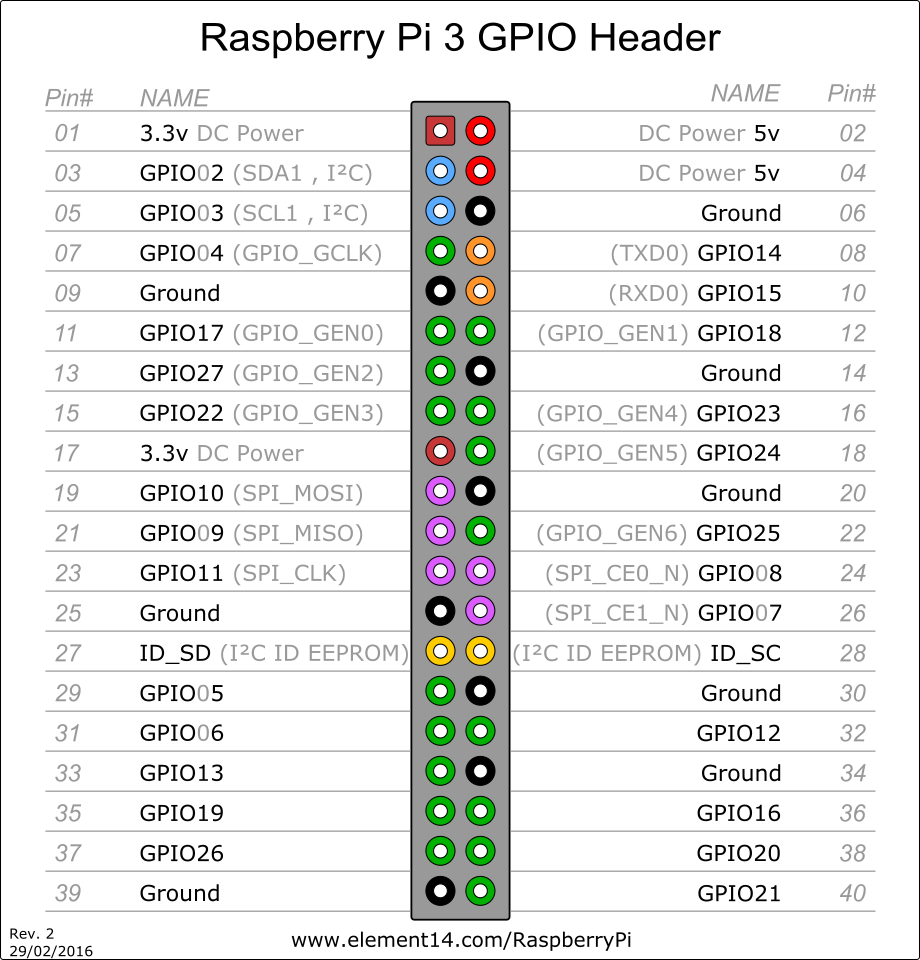
\includegraphics{images/gpio}
	}
	\caption{Le GPIO du Raspberry Pi 3}
	\label{img_gpio}
\end{figure}
\end{center}

\end{frame}

\begin{frame}[containsverbatim]
\frametitle{Le GPIO}

Vous pouvez remarquer qu'il y a des alimentations de 3,3V et de 5V (pin 01, 02, 04, 17) selon les périphériques que vous voulez brancher. Et Il y a des masses \emph{Ground}.

Les autres broches sont sur du courants de 3,3V. Le courant en sortie peut varier de 2 à 16mA. 

\end{frame}

\begin{frame}[containsverbatim]
\frametitle{Le GPIO}

Le GPIO permet de soit de contrôler soi même des éléments électroniques soit de mettre des extensions (HAT) pour avoir des périphériques. Vous en aurez à disposition le jour de l'atelier en petit nombre.

Le plus simple pour gérer ces sorties est le langage Python. Une bibliothèque Python est fourni pour contrôler le GPIO et aussi les périphériques qu'on branche dessus (le plus souvent).

Sinon vous avez la possibilité de contrôler le GPIO via un programme en C.

\end{frame}

\subsection{Eclairer une diode}

\begin{frame}[containsverbatim]
\frametitle{Une diode}

C'est la partie que je maitrise pas trop, c'est la partie électronique.

\end{frame}

\begin{frame}[containsverbatim]
\frametitle{L'aveu}

Pour allumer une diode, il faut mettre la résistance adéquate pour ne pas griller la diode. Pour une tension de 3,3V et avec une diode qui fait baisser la tension de 0,7V il faut absorber $3,3-0,7=2,6V$. Avec la loi d'Ohms, $U=R/I$, on calcule pour un courant de 5mA la résistance nécessaire~: $2,6/(5/1000)=520 ohms$. La résistance la plus proche est de 570 ohms. 

Il faut chercher la résistance qui va bien. Installer fil, diode et résistance sur la breadboard.

\end{frame}

\begin{frame}[containsverbatim]
\frametitle{Une diode}

Ensuite le programme Python est assez simple~:
\begin{verbatim}
import Rpi.GPIO as GPIO
import time
...
\end{verbatim}

\end{frame}

\begin{frame}[containsverbatim]
\frametitle{Une diode}

Pour faire un programme qui va faire clignoter indéfiniment la diode.

\begin{verbatim}
import Rpi.GPIO as GPIO
import time

GPIO.setmode(GPIO.BCM)
GPIO.setup(18, GPIO.OUT)

while TRUE:
...
\end{verbatim} 

\end{frame}

\begin{frame}[containsverbatim]
\frametitle{Une diode}

Attention en l'arrêtant avec controle+C vous allez laisser la broche dans un état ambigu.

Il vaut mieux quitter proprement~:

\begin{verbatim}
import Rpi.GPIO as GPIO
import time

GPIO.setmode(GPIO.BCM)
GPIO.setup(18, GPIO.OUT)

while TRUE:
    try:
...
\end{verbatim}

\end{frame}

 \subsection{PiFaceCAD}

 \begin{frame}[containsverbatim]
\frametitle{Le PiFaceCAD}
 
 Le PiFace est une carte avec un afficheur deux lignes 16 caractères, des boutons poussoirs et un un capteur infra-rouge.
 
Pour l'utiliser il faut activer la sortie SPI dans `raspi-config', redémarrer puis installer le paquet python-piface.

\begin{verbatim}
$sudo apt-get install python-pifacecad
\end{verbatim}
 
 \end{frame}
 
 \begin{frame}[containsverbatim]
\frametitle{Le PiFaceCAD}
 
 \begin{verbatim}
import pifacecad
import time
import netifaces as ni
...
\end{verbatim}

\end{frame}

\begin{frame}[containsverbatim]
\frametitle{Le PiFaceCAD}
 
Pour utiliser les boutons poussoirs, on crée un processus qui va surveiller et faire un ``goto'' dans une fonction pour traiter l'information.

\begin{verbatim}
import pifacecad
import time

...
\end{verbatim}

\end{frame}


\subsection{Sense HAT}

\begin{frame}[containsverbatim]
\frametitle{Sense HAT}

Il s'agit d'un ``chapeau'' ayant comme capteur~:
\begin{itemize}
    \item Gyroscope
    \item Accélèrometre
    \item Magnetomètre
    \item Capteur de temperature
    \item Capteur d'humidité
    \item Capteur de pression barometric
\end{itemize}
\end{frame}

\begin{frame}[containsverbatim]
\frametitle{Sense HAT}

Il possède aussi un affichage avec une matrice de 8x8 en RGB.

Il est célèbre pour avoir voyagé dans l'espace.

\end{frame}

\begin{frame}[containsverbatim]
\frametitle{Sense HAT}

Ci-dessous un script pour stocker dans un fichier l'humidité et la température que j'utilise chez moi.

\begin{verbatim}
#!/usr/bin/python
import sys
import os
import datetime

from sense_hat import SenseHat
...
\end{verbatim}

\end{frame}
\section{Application avec la caméra}

\subsection{Description des caméras}

Les caméras Pi sont de deux générations, les premières ont un capteur de 3 millions de pixels et les secondes de 5 millions.

Attention quand vous manipulez ces caméras, elle sont très sensibles à l'électricité statique. Par conséquent avant de les prendre en main il faut toucher un objet à la terre comme la cage de votre ordinateur ou un radiateur.

Elles se branchent sur le port CSI, entre le port HDMI et le jack audio/video. Les parties conductrices du ruban doivent se trouver vers la prise HDMI.

Il y a deux types de caméras~:
\begin{itemize}
	\item la caméra standard. C'est une caméra qui prend des photos ou vidéos que dans le visible.
	\item la caméra IR. C'est une caméra qui peut capturer des infra-rouges. Attention il faut une source de lumière adaptée comme des LEDs infra-rouges ou un dispositif pour les caméras extérieures. Quand la lumière dans le visible est forte elle capture le ``visible'' comme la caméra standard. Elle a donc un double usage.
\end{itemize}

Pour activer la caméra il faut lancer ``raspi-config'' et dans le menu activer la caméra.

\subsection{Capturer des images}

Le programme pour capturer des images s'appelle raspistill. 

pour capturer une image il suffit de faire~:

\begin{verbatim}
raspistill -o testcapture.jpg
\end{verbatim}

Pour régler la définition, il y a les arguments ``w'' et ``h''.

\begin{verbatim}
raspistill -w 1920 -h 1080 -o fullhdcapture.jpg
\end{verbatim}

Attention il y a un temps de latence avant la prise de vue ! Par défaut ce temps est de 5 secondes.

Pour éliminer ce temps de latence il faut utiliser le paramètre ``t''. Le temps à indiquer est un entier en millisecondes.

\begin{verbatim}
# pas de temps de latence
raspistill -t 1 -o tensecondcapture.jpg
# temps de latence d'une minute
raspistill -t 60000 -o tensecondcapture.jpg
\end{verbatim}

Le voyant de la caméra est rouge quand on prends un cliché.

\subsection{Capturer des vidéos}

Cette fois la commande est ``raspivid''. Par défaut elle encode en h264, un format propriétaire.

\begin{verbatim}
raspivid -o testvideo.h264
\end{verbatim}

Le temps de capture par défaut est de 5 secondes. 

Pour le modifier, il suffit d'utiliser l'argument ``t'' toujours en millisecondes

\begin{verbatim}
raspivid -t 60000 -o testvideo.h264
\end{verbatim}

Pour changer la résolution ce sont les mêmes arguments que pour ``raspistill''~:

\begin{verbatim}
raspivid -w 1280 -h 720 -t 60000 -o testvideo.h264
\end{verbatim}

Selon les modèles de caméras, les possibilités en matière de définition varient.

\subsection{Timelapse video}

Vous pouvez programmer la caméra pour prendre des photos à intervalle régulier. Par exemple pour prendre durant une minute une image toutes les secondes~:
\begin{verbatim}
raspistill -o frame%08d.jpg -tl 10000 -t 600000
\end{verbatim}

Dans ce cas vous verrez des fichiers appelés frame00000001.jpg, frame00000002.jpg, etc. dans le répertoire courant.

Pour les transformer en vidéo, il faut utiliser un utilitaire ``avconv''. Pour l'installer~:

\begin{verbatim}
$sudo apt-get install libav-tools
\end{verbatim}

Ensuite~:

\begin{verbatim}
avconv -r 10 -i frame%08d.jpg -r 10 -vcodec libx264 timelapse.mp4
\end{verbatim}

L'argument r indique le nombre de frames par secondes. L'argument vcodec indique le type de compression.

``avconv'' est un outil très complexe avec lequel on peut beaucoup de choses.


\end{document}
